% !TeX program = xelatex
\documentclass[UTF8,a4paper,11pt,fontset=windows]{ctexart}
\usepackage[left=18mm,right=18mm,top=16mm,bottom=17mm,headheight=14pt]{geometry}
\usepackage{amsmath,amssymb,array,booktabs,longtable,needspace,fancyhdr,xcolor,tikz}
\usepackage[hidelinks]{hyperref}
\setlength{\parindent}{0pt}\setlength{\parskip}{3pt}\linespread{1.1}
\setlength{\emergencystretch}{2em}\raggedbottom
\pagestyle{fancy}\fancyhf{}\renewcommand{\headrulewidth}{0pt}
\fancyfoot[C]{\small\PaperName\quad 第\thepage 页}
\newcommand{\R}{\mathbb R}
\newcommand{\blank}{\underline{\hspace{2.9cm}}}
\newcommand{\src}[1]{\par{\scriptsize\color{black!65}教材改编出处：#1。}\par}
\newcommand{\q}[2]{\par\Needspace{4\baselineskip}\textbf{#1.}\ #2}
\newcommand{\subq}[2]{\par\Needspace{2\baselineskip}（#1）#2}
\newcommand{\opts}[4]{\par\begin{tabular*}{\linewidth}{@{}p{.48\linewidth}@{\extracolsep{\fill}}p{.48\linewidth}@{}}A. #1&B. #2\\C. #3&D. #4\end{tabular*}\par}
\newcommand{\optsfour}[4]{\par\begin{tabular*}{\linewidth}{@{}p{.235\linewidth}@{\extracolsep{\fill}}p{.235\linewidth}p{.235\linewidth}p{.235\linewidth}@{}}A. #1&B. #2&C. #3&D. #4\end{tabular*}\par}
\newcommand{\parttitle}[1]{\par\Needspace{4\baselineskip}{\bfseries #1}\par}
\newcommand{\work}[1]{\par\vspace*{#1}}
\newcommand{\ans}[2]{\par\Needspace{4\baselineskip}\textbf{第#1题}\quad #2\par}
\newcommand{\readinggraph}{\begin{center}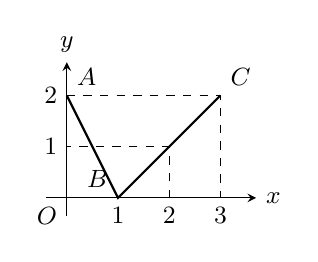
\begin{tikzpicture}[x=.65cm,y=.65cm,>=stealth,font=\small]
\draw[->](-.4,0)--(3.7,0)node[right]{$x$};\draw[->](0,-.35)--(0,2.65)node[above]{$y$};
\draw[thick](0,2)node[above right]{$A$}--(1,0)node[above left]{$B$}--(3,2)node[above right]{$C$};
\draw[dashed](0,2)--(3,2)--(3,0);\draw[dashed](2,0)--(2,1)--(0,1);
\node[below left]at(0,0){$O$};\foreach \x in {1,2,3}\node[below]at(\x,0){$\x$};
\foreach \y in {1,2}\node[left]at(0,\y){$\y$};\end{tikzpicture}\end{center}}
\renewcommand{\arraystretch}{1.2}

\newcommand{\PaperName}{C卷参考答案与评分}
\begin{document}
\begin{center}{\Large\bfseries 高一数学期中教材改编练习卷（C）}\\[2mm]参考答案、评分细则与教材出处\end{center}
单选、填空每题5分；多选全对6分，部分选对且无错项3分，含错项或未选0分。以下评分为本练习卷统一约定；解答题其他正确解法按相应步骤给分。
\parttitle{答案速查}\begin{center}\begin{tabular}{c|cccccccc}\toprule 题号&1&2&3&4&5&6&7&8\\答案&D&C&B&A&D&C&B&A\\\bottomrule\end{tabular}\par\smallskip\begin{tabular}{c|cccccc}\toprule 题号&9&10&11&12&13&14\\答案&AB&BC&AB&$[-3,3]$&$1$&$[-1,3]$\\\bottomrule\end{tabular}\end{center}
\parttitle{单项选择题解析}
\ans{1}{\textbf{D}。$\complement_U B=(-\infty,1]\cup(5,+\infty)$，再与A取交得 $[-1,1]$；1属于补集，不能漏掉。}
\ans{2}{\textbf{C}。两者均等价于 $-2\le x\le2$，可互相推出，为充要条件。}
\ans{3}{\textbf{B}。全称改存在，量词范围仍为 $[1,+\infty)$，$\ge1$ 的否定为 $<1$。}
\ans{4}{\textbf{A}。由 $x+(8-x)=8$，两项均为正，$x(8-x)\le16$，故根式不超过4；当 $x=4$ 时取等号。}
\ans{5}{\textbf{D}。A两者定义域分别为 $[0,+\infty)$ 和 $\R$；B第二个函数在0无定义；C对应关系不同（如x为负数）；D定义域均为 $\R$，展开后相同。}
\ans{6}{\textbf{C}。同时满足 $x\ge1$ 且 $x\ne3$，故为 $[1,3)\cup(3,+\infty)$。}
\ans{7}{\textbf{B}。$f(-2)=-5$，故所求为 $5+2(-5)=-5$。}
\ans{8}{\textbf{A}。整个区间在对称轴 $x=2$ 左侧，函数递减；故最小值为 $f(1)=1$。顶点不在给定区间内，不能答0。}
\parttitle{多项选择题与填空题解析}
\ans{9}{\textbf{AB}。乘以负数c反向，A正确；同加c保序，B正确；$a^2>b^2$，乘c后应为 $a^2c<b^2c$，C错误；$a/b>1$，D错误。}
\ans{10}{\textbf{BC}。定义域 $[-1,3]$ 不关于原点对称，故不是偶函数；另有 $f(-1)=2\ne f(1)=0$。其最小值0在1取得，最大值2在两个端点取得；在 $[-1,1]$ 上递减，$[1,3]$ 上递增。故B、C正确。}
\ans{11}{\textbf{AB}。由 $f(0)=0$ 及正半轴严格递增得 $f(2)>0$，B正确。又 $f(-3)=-f(3)<-f(1)=f(-1)$，A正确。$f(-2)<0<f(1)$，故C错误；非零且递增的奇函数不满足D，取x=1即见。}
\ans{12}{\textbf{$[-3,3]$}。配方得 $(x+m)^2+9-m^2$，最小值为 $9-m^2$，非负当且仅当 $m^2\le9$，故两个端点均可取。}
\ans{13}{\textbf{$1$}。由图得 $f(0)=2$。在线段BC上，$f(x)=x-1\ (1\le x\le3)$，所以 $f(2)=1$，故 $f(f(0))=1$。不能把f(0)的结果当作最终答案。}
\ans{14}{\textbf{$[-1,3]$}。$f(x)=(x-1)^2-1$，在 $[-1,1]$ 上，$(x-1)^2$ 取遍 $[0,4]$，故该段值域为 $[-1,3]$；在 $[1,2]$ 上值域为 $[-1,0]$。两者取并集得 $[-1,3]$。}

\newpage
\parttitle{解答题解析与分步评分}
\ans{15}{（15分）\subq{1}{$A\cap B=[-1,2]$（3分），$A\cup B=(-3,+\infty)$（3分），$\complement_U A=(-\infty,-3]\cup(2,+\infty)$（3分）。}\subq{2}{若 $t\le-3$，则对任意 $x\in A$，均有 $x>-3\ge t$，故包含关系成立（3分）。若 $t>-3$，当 $t\le2$ 时可取 $x=(-3+t)/2\in A$ 且 $x<t$；当 $t>2$ 时可取 $x=2\in A$ 且 $x<t$。故必须且只需 $t\le-3$（3分）。}}
\src{p.13，习题1.1第9题；p.13，习题1.1第16题}
\ans{16}{（15分）\subq{1}{原式等价于 $-3\le2x-1\le3$（3分），故解集为 $[-1,2]$（3分）。}\subq{2}{原式等价于 $(x-m)(x-3)>0$（3分）。当 $m<3$ 时，解集为 $(-\infty,m)\cup(3,+\infty)$（2分）；当 $m=3$ 时，解集为 $\R\setminus\{3\}$（2分）；当 $m>3$ 时，解集为 $(-\infty,3)\cup(m,+\infty)$（2分）。}}
\src{p.59，习题2.3第4题；p.59，习题2.3第8题}
\ans{17}{（17分）\subq{1}{定义域关于原点对称（1分），$f(-x)=g(-x)+g(x)=f(x)$（2分），所以为偶函数（1分）。}\subq{2}{当 $x\in[-3,0)$ 时，$-x\in(0,3]$（1分），$f(-x)=x^2+4x+1$（2分），由偶性 $f(x)=x^2+4x+1$（2分）。}\subq{3}{在 $[0,3]$ 上 $f(x)=(x-2)^2-3$（2分），最小值为 $-3$；端点值 $f(0)=1,f(3)=-2$，最大值为1（各1分）。结合偶性，最小值 $-3$ 在 $x=\pm2$ 时取得（2分），最大值1仅在 $x=0$ 时取得（2分）。}}
\src{p.84，例5；p.90，复习题第7题}
\ans{18}{（17分）\subq{1}{$81^{3/4}=27$（2分），$25^{-1/2}=1/5$，原式为 $136/5$（2分）。}\subq{2}{由 $9^\alpha=27=9^{3/2}$ 得 $\alpha=3/2$（2分），$f(x)=x^{3/2}=x\sqrt x$（1分），定义域为 $[0,+\infty)$（2分）。}\subq{3}{定义域不关于原点对称，既不是奇函数也不是偶函数（2分）；在 $[0,+\infty)$ 上递增（2分）。任取 $0\le x_1<x_2$（1分），$f(x_2)-f(x_1)=(\sqrt{x_2}-\sqrt{x_1})(x_2+\sqrt{x_1x_2}+x_1)>0$（2分），故在定义域上严格递增（1分）。}}
\src{p.104，习题4.1第4题；p.104，习题4.1第8题}
\ans{19}{（13分）\subq{1}{由 $100a^2=25$ 得 $a=1/2$（2分），故 $M(t)=100(1/2)^t\ (t\ge0)$（1分）。}\subq{2}{底数在0与1之间，故在 $[0,+\infty)$ 上严格递减（2分）；最大值100在 $t=0$ 时取得，且 $t$ 增大时可无限接近0，值域为 $(0,100]$（2分）；任意有限时间指数幂恒为正，剩余量不等于0（2分）。}\subq{3}{原式等价于 $(1/2)^t\ge(1/2)^3$，故 $t\le3$（2分）；结合 $t\ge0$ 得 $t\in[0,3]$（2分）。}}
\src{p.112，例6；p.108，练习第2题}

\newpage
\parttitle{命题结构与教材改编记录}
本卷只使用教材第1至3章及第4章4.1至4.2的例题、习题和练习作为母题。集合与逻辑30分，不等式31分，函数概念与性质59分，幂函数与指数函数30分；合计150分。
\par 主考点归类：集合1、15题共20分，逻辑2、3题共10分；基本不等式4题5分、不等式性质9题6分、恒成立12题5分、二次不等式16题15分；函数概念5、6、13题共15分，函数性质7、8、10、11、14、17题共44分；幂函数18题17分、指数函数19题13分。综合题允许知识交叉，归类用于统计，不将同一分数重复计入。
\par 教材页码指印刷页，正文PDF页序为印刷页加7。下列ID均可在教材题库中检索，改编题的答案已另行重算，不能直接套用母题答案。
\par 未特别注明的改编均为更换数据与设问、保留教材母题的概念结构。逐题目标、预期方法、易错点及评价方式另见随附“命题细目与教材出处.csv”。
\small\begin{longtable}{@{}p{.045\linewidth}p{.925\linewidth}@{}}\toprule 题号&教材母题与改编说明\\\midrule\endhead
1 & p.13，习题1.1第9题（PDF第20页）\newline{\scriptsize\ttfamily\detokenize{XJ-B1-C01-HW-P013-Y0433}}\\[3pt]
2 & p.18，例5（PDF第25页）\newline{\scriptsize\ttfamily\detokenize{XJ-B1-C01-EX-P018-Y0491}}\\[3pt]
3 & p.23，页首练习（PDF第30页）\newline{\scriptsize\ttfamily\detokenize{XJ-B1-C01-PR-P023-Y0176}}\\[3pt]
4 & p.43，习题2.1第7题（PDF第50页）\newline{\scriptsize\ttfamily\detokenize{XJ-B1-C02-HW-P043-Y1506}}\\[3pt]
5 & p.77，习题3.1第5题（PDF第84页）\newline{\scriptsize\ttfamily\detokenize{XJ-B1-C03-HW-P077-Y0403}}\\[3pt]
6 & p.77，习题3.1第4题（PDF第84页）\newline{\scriptsize\ttfamily\detokenize{XJ-B1-C03-HW-P077-Y0286}}\\[3pt]
7 & p.86，习题3.2第6题（PDF第93页）\newline{\scriptsize\ttfamily\detokenize{XJ-B1-C03-HW-P086-Y0231}}\\[3pt]
8 & p.82，练习第2题（PDF第89页）\newline{\scriptsize\ttfamily\detokenize{XJ-B1-C03-PR-P082-Y1193}}\\[3pt]
9 & p.37，练习第1题（PDF第44页）\newline{\scriptsize\ttfamily\detokenize{XJ-B1-C02-PR-P037-Y0875}}\\[3pt]
10 & p.75，例7（PDF第82页）\newline{\scriptsize\ttfamily\detokenize{XJ-B1-C03-EX-P075-Y0177}}\\[3pt]
11 & p.86，习题3.2第10题（PDF第93页）\newline{\scriptsize\ttfamily\detokenize{XJ-B1-C03-HW-P086-Y0853}}\\[3pt]
12 & p.55，例5（PDF第62页）\newline{\scriptsize\ttfamily\detokenize{XJ-B1-C02-EX-P055-Y0177}}\\[3pt]
13 & p.78，习题3.1第14题（PDF第85页）\newline{\scriptsize\ttfamily\detokenize{XJ-B1-C03-HW-P078-Y0808}}\newline 改编：将教材折线图函数复合求值题更换顶点坐标并减少复合层数，保留按图读取对应关系。\\[3pt]
14 & p.90，复习题第7题（PDF第97页）\newline{\scriptsize\ttfamily\detokenize{XJ-B1-C03-RV-P090-Y1256}}\\[3pt]
15 & p.13，习题1.1第9题（PDF第20页）；p.13，习题1.1第16题（PDF第20页）\newline{\scriptsize\ttfamily\detokenize{XJ-B1-C01-HW-P013-Y0433 / XJ-B1-C01-HW-P013-Y1442}}\\[3pt]
16 & p.59，习题2.3第4题（PDF第66页）；p.59，习题2.3第8题（PDF第66页）\newline{\scriptsize\ttfamily\detokenize{XJ-B1-C02-HW-P059-Y0221 / XJ-B1-C02-HW-P059-Y0874}}\\[3pt]
17 & p.84，例5（PDF第91页）；p.90，复习题第7题（PDF第97页）\newline{\scriptsize\ttfamily\detokenize{XJ-B1-C03-EX-P084-Y0592 / XJ-B1-C03-RV-P090-Y1256}}\\[3pt]
18 & p.104，习题4.1第4题（PDF第111页）；p.104，习题4.1第8题（PDF第111页）\newline{\scriptsize\ttfamily\detokenize{XJ-B1-C04-HW-P104-Y0874 / XJ-B1-C04-HW-P104-Y1494}}\\[3pt]
19 & p.112，例6（PDF第119页）；p.108，练习第2题（PDF第115页）\newline{\scriptsize\ttfamily\detokenize{XJ-B1-C04-EX-P112-Y1015 / XJ-B1-C04-PR-P108-Y1402}}\newline 改编：融合放射性物质衰减例题与半衰期练习，指定指数模型，更换初始量及观测值，增加模型定义域和非零性的解释。\\[3pt]
\bottomrule\end{longtable}\normalsize
\par\textbf{评价与复习建议：}客观题逐项判断，填空题核对端点和可取性；解答题按列式、推理、分类完整性及结论评分。第17、18题重点观察能否从定义出发说明理由。上述难度与错误仅为教学预判，未经过班级试测，不预设均分或达标率。
\end{document}
